
\section{Inéquations à une inconnue}


\subsection{Inéquations du premier degré}

$ 2x - 5 \leqslant 0 $\\

$2x \leqslant 5 $\\

$ x \leqslant \dfrac{5}{2} $\\ 

Résoudre l'inéquation $ 2x-5\leqslant 0 $, c'est trouver l'ensemble des nombres réels x tels que :\\

$ 2x -5 \leqslant 0 $.

\vspace*{-.3cm}
\begin{tikzpicture}
     \tkzInit[xmin=-30,xmax=20,xstep=6]
     \tkzDrawX[label={},noticks,nograd]
     
     \tkzXHW    % I=]-10,7[
     {
%      -30/T//-10/T/],        % On hachure  de -inf à -10
        7/T/[/20/T/          % et de 9 à +inf
     }
%     \tkzText(-10,-.5){a}    % Etiquette gauche
     \tkzText(6.5,.6){$\dfrac{5}{2}$}      % Etiquette droite
%     \tkzText(0,0){\textcolor{red}{$\times$}}  % Etiquette croix sur R
%     \tkzText(0,-.3){\textcolor{red}{$x$}}     % Etiquette x sous croix
\end{tikzpicture}

$ S = \left]-\infty ; \dfrac{5}{2}\right[ $ \\

Néanmoins, il faut faire attention, car parfois, le sens se modifie : \\

$ -3x + 7 < 0 $\\

$ -3x < -7 $\\

$ 3x > 7 $\\

$ x > \dfrac{7}{3} $ 

\vspace*{-.3cm}
\begin{tikzpicture}
     \tkzInit[xmin=-30,xmax=20,xstep=6]
     \tkzDrawX[label={},noticks,nograd]
     
     \tkzXHW {
      -30/T//-10/T/]        % On hachure  de -inf à -10
%        7/T/[/20/T/          % et de 9 à +inf
     }
     \tkzText(-9.5,.6){$\dfrac{7}{3}$}    % Etiquette gauche
%     \tkzText(6.5,.6){$\dfrac{5}{2}$}      % Etiquette droite
%     \tkzText(0,0){\textcolor{red}{$\times$}}  % Etiquette croix sur R
%     \tkzText(0,-.3){\textcolor{red}{$x$}}     % Etiquette x sous croix
\end{tikzpicture}

\hspace*{4cm}$ S = \left]\dfrac{7}{3}, +\infty\right[ $ \\

\textbf{Attention à certaines inéquations}

$ 2x + 3 \leqslant x + 1 + x + 7 $\\

$ 2x - 2x \leqslant 1 + 7 - 3 $\\

$ 0x \leqslant 5 $ \\

Toujours vrai, donc : $ S = \R = \left]-\infty, +\infty\right[ $ \\

\newpage 

\textbf{Remarque}

Pour les 3 autres équations de la même famille, on aurait : 

$ 0x < 5 $ donne $ S = \R = \left]-\infty, +\infty\right[ $\\

$ 0x > 5 $ donne $ S = \varnothing $\\

$ 0x \geqslant 5 $ donne $ S = \varnothing $ \\

Pour $ 3 + 5x > 2 + 3x + 1 + 2x $, on a :\\

$ -3x - 2x + 5x > 1 + 2 - 3 $\\

$ 0x > 0 $ 

Impossible, donc $ S = \varnothing $ \\

\newpage 
\subsection{Signe de $\mathbf{ax+b}$ (Tableau de signes)}

\begin{tabular}{rl}
Soit : & $ f : \R \rightarrow \R$\\
& $ x\mapsto f(x) = ax + b $ avec $ a \neq 0 $ \\
&\\
& \textbf{Remarque}\\
& La fonction $f$ est une fonction affine, car $ f(x) = ax + b $\\
\end{tabular}

\subsubsection{Exemple \no 1}

Si $ f(x) = 2x-5 $ avec $a = 2$ et $b = -5$, on a : \\

\begin{tabular}{ccc}

$f(x) = 0$ & $f(x) < 0 $ & $f(x) > 0$ \\
\\
$2x - 5 = 0$ & $2x - 5 < 0$ & $2x - 5 > 0$ \\
$2x = 5 $ & $ 2x < 5 $ & $2x > 5 $ \\
$ x = \dfrac{5}{2} $ & $x <\dfrac{5}{2}$ & $x>\dfrac{5}{2}$ \\
\end{tabular}\\


\begin{tikzpicture} 

\tkzTabInit[lgt=2,espcl=1] 
{ $x$         /1, 
$2x-5$   /1}
{$ - \infty $ , $ \dfrac{5}{2} $ , $ + \infty $}
\tkzTabLine{ , - , z , + , }

\end{tikzpicture} 


\subsubsection{Exemple \no 2}

$ f(x) = -3x + 7 $ \\

\begin{tabular}{ccc}

$f(x) = 0$ & $f(x) < 0 $ & $f(x) > 0$ \\

$-3x +7 = 0$ & $-3x +7 < 0$ & $-3x +7 > 0$ \\
$-3x = -7 $ & $ -3x < -7 $ & $-3x > -7 $ \\
$ x = \dfrac{7}{3} $ & $x >\dfrac{7}{3}$ & $x<\dfrac{7}{3}$ \\
\end{tabular}

\begin{tikzpicture} 

\tkzTabInit[lgt=2,espcl=1] 
{ $x$         /1, 
$-3x+7$   /1}
{$ - \infty $ , $ \dfrac{7}{3} $ , $ + \infty $}
\tkzTabLine{ , + , z , - , }

\end{tikzpicture} 

\subsubsection{Tableau récapitulatif}

$ f(x) = ax + b $ avec $ a \neq 0 $ 

$ ax + b = 0 $

$ax = -b $

$ x = -\dfrac{b}{a} $

\vspace {.5cm}

\begin{tikzpicture} 

\tkzTabInit[lgt=4,espcl=3] 
{ $x$ /1, 
$ax+b$  /1}
{$ - \infty $ , $-\dfrac{b}{a} $ , $ + \infty $}
\tkzTabLine{ , $Signe de $-a$$ , z , $Signe de $a$$ }
\end{tikzpicture} 


\subsection{Inéquations produit}

\subsubsection*{Comment faire ?}

\textbf{Exemple \no 0}

$ \left(2x + 5\right)\left(-3x + 7\right) \leqslant 0 $ \\

Il faut faire un tableau de signes : \\

\begin{tikzpicture}

\tkzTabInit[lgt=3,espcl=2]
{ $x$  /1,
$2x+5$   /1,
$-3x + 7$ /1,
$\left(2x+5\right)\left(-3x+7\right)$ /1}
{$ - \infty $ , $-\dfrac{5}{2} $ , $\dfrac{7}{3} $ , $ + \infty $}
\tkzTabLine{ , - , z , +, t  ,+  }
\tkzTabLine{ , + , t , + , z, - }
\tkzTabLine{ , - , z , +, z, - }
\draw[decoration={brace, mirror, raise=0.2cm}, decorate, line width=2pt,black] (T14) -- (N24) ;
\draw[decoration={brace, mirror, raise=0.2cm}, decorate, line width=2pt,black] (N34) -- (T24) ;
\end{tikzpicture}
\\

\begin{tabular}{ccc}
$2x-5=0$& et &$-3x + 7 = 0$ \\
\\
$2x = -5$& et &$-3x = 7 $ \\
\\
$x= -\dfrac{5}{2}$& et & $x=\dfrac{7}{3}$ \\
\end{tabular}\\

\vspace{.1cm}

$ S = \left]-\infty, -\dfrac{5}{2}\right]\cup\left[\dfrac{7}{3},+\infty\right[ $ \\

\textbf{Exemple \no 1}\\

$ x^2 - 9 \leqslant 0 $\\

$ \left(x+3\right)\left(x-3\right) \leqslant 0 $\\

\begin{tabular}{lcl}

$x+3$ & ou & $ x - 3 = 0 $ \\
$x=-3$ & ou & $ x = 3 $ \\
\end{tabular}

\vspace{.5cm}

\begin{tikzpicture}
\tkzTabInit[lgt=3,espcl=2] 
{ $x$        /1 , 
$x+3$ /1 ,
$x-3$ /1,
$\left(x+3\right)\left(x-3\right)$ /1}
{$ -\infty $ , $-3 $ , $3$ , $ +\infty $}
\tkzTabLine{ , - , z , +, t  ,+  }
\tkzTabLine{ , - , t , - , z, + }
\tkzTabLine{ , + , z , -, z, + }
\end{tikzpicture} 

\newpage

\textbf{Exemple \no 2}

$ -x^2+5x < 0 $\\

$ x\left(-x+5\right) = 0$\\

\vspace{.5cm}

\begin{tikzpicture}
\tkzTabInit[lgt=3,espcl=2] 
{ $x$        /1 , 
$x$        /1 , 
$-x+5$ /1 ,
$x\left(-x+5\right)$ /1}
{$ -\infty $ , $0 $ , $5$ , $ +\infty $}
\tkzTabLine{ , - , z , +, t  ,+  }
\tkzTabLine{ , + , t , + , z, - }
\tkzTabLine{ , - , z , +, z, - }
\draw[decoration={brace, mirror, raise=0.2cm}, decorate, line width=2pt,black] (T14) -- (N24) ;
\draw[decoration={brace, mirror, raise=0.2cm}, decorate, line width=2pt,black] (N34) -- (T24) ;
\end{tikzpicture}
\\


$ S = \left]-\infty, 0 \right[\cup\left]5, +\infty\right[ $ \\

\textbf{Exercice \no 1}\\

$ x^2+24x-52 \geqslant 0 $

... 

$ \left(x+26\right)\left(x-2\right) \geqslant 0 $ \\

\begin{tabular}{ccc}
$x+26$ & ou & $x-2 = 0$ \\
$x=-26$ & ou &$x=2$ \\
\end{tabular}

\vspace{.5cm}

\begin{tikzpicture}

\tkzTabInit[lgt=3,espcl=2]
{ $x$  /1,
$x+26$   /1,
$x-2$ /1,
$\left(x+26\right)\left(x-2\right)$ /1}
{$ - \infty $ , $-26 $ , $2 $ , $ + \infty $}
\tkzTabLine{ , - , z , +, t  ,+  }
\tkzTabLine{ , - , t , - , z, + }
\tkzTabLine{ , + , z , -, z, + }
\draw[decoration={brace, mirror, raise=0.2cm}, decorate, line width=2pt,black] (T14) -- (N24) ;
\draw[decoration={brace, mirror, raise=0.2cm}, decorate, line width=2pt,black] (N34) -- (T24) ;
\end{tikzpicture}
\\

$ S = \left]-\infty, -26\right]\cup\left[2, +\infty\right[ $ \\


\newpage 

\textbf{Exercice \no 2}\\

$-9x^2+21x+8 > 0 $

...

$ \left(3x+1\right)\left(3x-8\right)<0 $

\begin{tabular}{ccc}
$3x + 1 = 0$ & ou & $3x - 8 = 0 $ \\
$x = -\dfrac{1}{3} $ & ou & $x=\dfrac{8}{3} $ \\
\end{tabular}\\

\begin{tikzpicture}
\tkzTabInit[lgt=3,espcl=2,]
{ $x$  /1,
$3x+1$   /1,
$3x - 8$ /1,
$\left(3x+1\right)\left(3x-8\right)$ /1}
{$ - \infty $ , $-\dfrac{1}{3} $ , $\dfrac{8}{3} $ , $ + \infty $}
\tkzTabLine{ , - , z , +, t  ,+  }
\tkzTabLine{ , - , t , - , z, + }
\tkzTabLine{ , + , z , -, z, + }
\draw[decoration={brace, mirror, raise=0.2cm}, decorate, line width=2pt,black] (N24) -- (N34) ;

\end{tikzpicture}

$ S = \left]-\dfrac{1}{3}, \dfrac{8}{3} \right[ $ \\

\textbf{Attentions à certaines inéquations}

\textbf{Exemple \no 1}\\

$ 49x^2 - 14x + 1 \leqslant 0 $\\

$ \left(7x-1\right)^2 \leqslant 0 $ \\

$ 7x - 1 = 0 $\\

$ 7x = 1 $\\

$ x = \dfrac{1}{7} $

\begin{tikzpicture}

\tkzTabInit[lgt=3,espcl=2]
{ $x$  /1,
$7x-1$   /1,
$7x-1$ /1,
$\left(7x-1\right)^2$ /1}
{$ - \infty $ , $\dfrac{1}{7} $ , $ + \infty $}
\tkzTabLine{ , - , z , +  }
\tkzTabLine{ , - , z , + }
\tkzTabLine{ , + , z , +, }
\end{tikzpicture}

$ S = \lb \dfrac{1}{7} \rb $ \\

\textbf{Remarque :}

Pour les 3 autres inéquations de la même famille, on aura :

\begin{tabular}{cc}
$49x^2 - 14x + 1 < 0$ & $S = \varnothing$ \\
$49x^2 - 14x + 1 \geqslant 0$& $ S = \R = \left]-\infty ; +\infty\right[$ \\
$49x^2 - 14x + 1 > 0$ & $ S = \left]-\infty ; \dfrac{1}{7} \right[\cup \left]\dfrac{1}{7}; +\infty\right[ $ \\
\end{tabular}

\newpage 

\textbf{Exemple \no 2} 

$ 25x^2 + 20x + 13 \leqslant 0 $\\

$ 25x^2 + 20x + 4 + 9 \leqslant 0 $\\

$ \left(5x + 2\right)^2 + 9 \leqslant 0 $\\

$ \left(5x + 2\right)^2 \leqslant - 9 $\\

Or, le carré d'un nombre est toujours positif. \\
Donc $ S = \varnothing $.\\

\textbf{Remarque :}

Pour les 3 autres inéquations de la même famille, on aura :

\begin{tabular}{cc}
$25x^2 + 20x + 13 < 0$ & $S = \varnothing$ \\
$25x^2 + 20x + 13 < 0$ & $ S = \R = \left]-\infty ; +\infty\right[$ \\
$25x^2 + 20x + 13 < 0$ & $ S = \R = \left]-\infty ; +\infty\right[$ \\
\end{tabular}

\newpage 
\subsection{Inéquation avec l'inconnue au dénominateur}

$ \dfrac{6}{x-2} \leqslant x-3 $\\

\textbf{Il ne faut pas que $ x-2 = 0 $ donc que $ x = 2 $}\\

\textbf{Valeur interdite : $ x = 2 $}\\

\textbf{Attention, dans le cas des inéquations, le produit en croix est interdit}\\

$ \dfrac{6}{x-2} - \left(x-3\right) \leqslant 0 $\\

$ \dfrac{6 - \left(x-2\right)\left(x-3\right)}{x-2} \leqslant 0 $\\

$ \dfrac{6 - \left(x^2 - 5x + 6 \right)}{x-2} \leqslant 0 $\\

$ \dfrac{-x^2 + 5x}{x-2} \leqslant 0 $\\

\vspace{.5cm}

\begin{tikzpicture}

\tkzTabInit[lgt=3,espcl=2,]
{ $x$  /1,
$x$ /1,
$-x+5$   /1,
$x -2 $ /1,
$\dfrac{x\left(-x+5\right)}{x-2}$ /1}
{$ - \infty $ , $0 $ , $2 $ , $5$ , $ + \infty $}
\tkzTabLine{ , - , z , +, t  ,+ , t , + }
\tkzTabLine{ , + , t , + , t , + , z, - }
\tkzTabLine{ , - , t , - , z , + , t , + }
\tkzTabLine{ , + , z , - , d , + , z , - }
\draw[decoration={brace, mirror, raise=0.2cm}, decorate, line width=2pt,black] (N25) -- (N35) ;
\draw[decoration={brace, mirror, raise=0.2cm}, decorate, line width=2pt,black] (N45) -- (T25) ;
\end{tikzpicture}
\\

$ S = \left[0,2\right[\cup \left[5, + \infty \right[ $ \\
\newpage
\textbf{Exercice \no 2} \\

$ \dfrac{x^2-15}{\left(x-4\right)\left(x-3\right)} \geqslant \dfrac{1}{x-4} - \dfrac{1}{x-3} $ \\

\textbf{Valeurs interdites : $x=4 $ et $ x = 3 $}  \\

$ \dfrac{x^2-15}{\left(x-4\right)\left(x-3\right)} \geqslant \dfrac{\left(x-3\right)-\left(x-4\right)}{\left(x-4\right)\left(x+3\right)} $ \\

$ \dfrac{x^2-15}{\left(x-4\right)\left(x-3\right)} \geqslant \dfrac{1}{\left(x-4\right)\left(x+3\right)} $ \\

$ \dfrac{x^2-15-1}{\left(x-4\right)\left(x-3\right)} \geqslant 0  $ \\

$ \dfrac{x^2-16}{\left(x-4\right)\left(x-3\right)} \geqslant 0  $ \\

$ \dfrac{\left(x+4\right)\left(x-4\right)}{\left(x-4\right)\left(x-3\right)} \geqslant 0  $ \\

\textbf{Remarque}

Simplifier est alors dangereux... Il est plus prudent d'écrire le tableau de signes ainsi : \\

\begin{tikzpicture}

\tkzTabInit[lgt=3,espcl=2]
{ $x$  /1,
$x+4$ /1,
$x-4$   /1,
$x-4 $ /1,
$x-3$ /1,
$\dfrac{x\left(x+4\right)\left(x-4\right)}{\left(x-4\right)\left(x-3\right)}$ /1}
{$ - \infty $ , $-4 $ , $3 $ , $4$ , $ + \infty $}
\tkzTabLine{ , - , z , +, t  ,+ , t , + }
\tkzTabLine{ , - , t , - , t , - , z, + }
\tkzTabLine{ , - , t , - , t , - , z, + }
\tkzTabLine{ , - , t , - , z , + , t , + }
\tkzTabLine{ , + , z , - , d , + , d , + }
\draw[decoration={brace, mirror, raise=0.2cm}, decorate, line width=2pt,black] (T16) -- (N26) ;
\draw[decoration={brace, mirror, raise=0.2cm}, decorate, line width=2pt,black] (N36) -- (N46) ;
\draw[decoration={brace, mirror, raise=0.2cm}, decorate, line width=2pt,black] (N46) -- (T26) ;
\end{tikzpicture}\\

$S=\left]-\infty,-4\right]\cup\left]3,4\right[\cup\left]4,+\infty\right[$

\newpage 
\subsection{Systèmes d'inéquations}

\subsubsection{Exemple \no 1}

\vspace*{.5cm}

\begin{minipage}{3cm}
\begin{equation*}
\left\lbrace \begin{aligned}
2x+3      &> 3x-2\\
3(x-2)    &\geqslant 2-5x\\
\end{aligned}
\right.
\end{equation*}
\end{minipage}

\vspace*{.5cm}

Résoudre un tel système, c'est trouver l'ensemble des nombres réels $x$ \\
tels que $ 2x + 3 > 3x - 2 $ 
\textbf{et} $ 3\left(x-2\right) \geqslant 2 -5x $\\

\textbf{1$^{re}$ inéquation :}\\

$2x + 3 > 3x - 2$\\

$- x > -5$\\

$x < 5$ \\

$ S_1 = \left]-\infty, 5 \right[ $ \\

\textbf{2$^{me}$ inéquation :}\\

$ 3\left(x-2\right) \geqslant 2 - 5x $\\

$ 3x - 5 \geqslant 2 - 5x $\\

$ 8 x \geqslant 8 $\\

$ x \geqslant 1 $ \\

$ S_2 = \left[1, +\infty\right[ $ \\

\textbf{3 : Système}\\

$ S = S_1 \cap S_2 $


\vspace*{-.3cm}
\begin{tikzpicture}
     \tkzInit[xmin=-30,xmax=20,xstep=6]
     \tkzDrawX[label={},noticks,nograd]
     
      \tkzDefPoint(-30,-.05){A1} 
      \tkzDefPoint(7,-.05){A2} 
     \tkzDrawSegment[color=green](A1,A2) ; 
       \tkzXHW [color=green]  % XHW : hachures SW -> NE  
     {
%      -30/T//-10/T/],        % On hachure  de -inf à -10
        7/T/[/20/T/          % et de 9 à +inf
     }
        
     \tkzDefPoint(-10,.05){B1} 
      \tkzDefPoint(20,.05){B2} 
     \tkzDrawSegment[color=red](B1,B2) ; 
     \tkzXH [color=red]   % XH : hachures NW -> SE
     {
      -30/T//-10/T/[        % On hachure  de -inf à -10
%        7/T/[/20/T/          % et de 9 à +inf
     }
     
     \tkzText(-10,.5){$1$}    % Etiquette gauche
     \tkzText(6.5,.6){$5$}      % Etiquette droite
%     \tkzText(0,0){\textcolor{red}{$\times$}}  % Etiquette croix sur R
%     \tkzText(0,-.3){\textcolor{red}{$x$}}     % Etiquette x sous croix
\end{tikzpicture}


$ S= \left[1,5\right[ $
\newpage
\subsubsection{Exemple \no 2}

\vspace*{.5cm}

\begin{minipage}{3cm}
\begin{equation*}
\left\lbrace \begin{aligned}
\dfrac{3}{5}x     &  >     \dfrac{1}{5} + x \\
6\left(2-x\right) & \leqslant   -2x \\
\end{aligned}
\right.
\end{equation*}
\end{minipage}

\vspace*{.5cm}

\textbf{1$^{re}$ inéquation :}

$ \dfrac{3}{5}x - x > \dfrac{1}{5} $\\

$ x \left(\dfrac{3}{5} - 1\right) > \dfrac{1}{5} $\\

$ -\dfrac{2}{5}x > \dfrac{1}{5} $\\

$ x < \dfrac{1}{5} \times \left(-\dfrac{5}{2}\right) $\\

$ x < -\dfrac{1}{2} $ \\

$ S_1 = \left]-\infty, -\dfrac{1}{2} \right[ $\\

\textbf{2$^{me}$ inéquation :}

$12 - 6x \leqslant -2x $\\

$ -4x \leqslant -12 $\\

$ 4x \geqslant 12 $\\

$ x \geqslant 3 $ \\

$ S_2 = \left[3, +\infty\right[ $\\

\textbf{3 : Système}\\

$ S = S_1 \cap S_2 = \varnothing $\\

\vspace*{-.3cm}
\begin{tikzpicture}   
     \tkzInit[xmin=-5,xmax=7]
     \tkzDrawX[label={},noticks,nograd]
     
      \tkzDefPoint(3,.1){A1} 
      \tkzDefPoint(7,.1){A2} 
     \tkzDrawSegment[color=red](A1,A2) ; 
       \tkzXH [color=red]  % XHW : hachures SW -> NE  
     {
        -5/T//3/T/[          % True de 3 à +inf 
     }
        
     \tkzDefPoint(-5,-.1){B1} 
      \tkzDefPoint(-1/2,-.1){B2} 
     \tkzDrawSegment[color=blue](B1,B2) ; 
     \tkzXHW [color=blue]   % XH : hachures NW -> SE
     {
      -.5/T/[/7/T/        % On hachure  de -inf à -10
     }
     
    \tkzText(-1/2,.5){$-\dfrac{1}{2}$}    % Etiquette gauche
    \tkzText(3,.6){$3$}      % Etiquette droite
\end{tikzpicture}

\textbf{Remarque}

Les 2 inéquations sont incompatibles.
\newpage 
\subsubsection{Exercice \no 1}

\begin{minipage}{3cm}
\begin{equation*}
\left\lbrace \begin{aligned}
4x^2 + 3x + 1&\geqslant x^2 - 3x + 1\\
\left(x+1\right)^2&> 5x+5 \\
\end{aligned}
\right.
\end{equation*}
\end{minipage}

\vspace{.5cm}

\textbf{1$^{re}$ inéquation}\\

$ 3x^2 + 6x \geqslant 0 $

$ 3x \left(x+2\right) \geqslant 0 $\\ 

\begin{tikzpicture}
\tkzTabInit[lgt=3,espcl=2]
{ $x$  /1,
$3x$ /1,
$x+2$   /1,
$3x\left(x+2\right)$ /1}
{$ - \infty $ , $-2 $ , $0 $ , $ + \infty $}
\tkzTabLine{ , - , t , -, z  ,+ }
\tkzTabLine{ , - , z , + , t , + }
\tkzTabLine{ , + , z , - , z , + }
\draw[decoration={brace, mirror, raise=0.2cm}, decorate, line width=2pt,black] (T14) -- (N24) ;
\draw[decoration={brace, mirror, raise=0.2cm}, decorate, line width=2pt,black] (N34) -- (T24) ;
\end{tikzpicture}


$ S_1 = \left]-\infty, -2\right]\cup[0,+\infty[ $ \\

\textbf{2$^{me}$ inéquation}\\

$ \left(x+1\right)^2 > 5\left(x+1\right) $

$ \left(x+1\right)^2 - 5\left(x+1\right)  > 0 $

$ \left(x+1\right)\left(x+1-5\right) > 0 $

$ \left(x+1\right)\left(x-4\right) > 0 $\\



\begin{tikzpicture}
\tkzTabInit[lgt=3,espcl=2]
{ $x$  /1,
$x+1$ /1,
$x-4$   /1,
$\left(x+1\right)\left(x-4\right)$ /1}
{$ - \infty $ , $-1 $ , $4 $ , $ + \infty $}
\tkzTabLine{ , - , z , +, t  ,+ }
\tkzTabLine{ , - , t , - , z , + }
\tkzTabLine{ , + , z , - , z , + }
\draw[decoration={brace, mirror, raise=0.2cm}, decorate, line width=2pt,black] (T14) -- (N24) ;
\draw[decoration={brace, mirror, raise=0.2cm}, decorate, line width=2pt,black] (N34) -- (T24) ;
\end{tikzpicture}\\

$ S_2 = \left]-\infty, -1\right[\cup\left]4, + \infty \right[ $\\

\textbf{3 : Système}

$ S = S_1 \cap S_2 = \left]-\infty, -2\right]\cup\left]4, + \infty\right[ $\\


\begin{tikzpicture}   
     \tkzInit[xmin=-5,xmax=7]
     \tkzDrawX[label={},noticks,nograd]
     
      \tkzDefPoint(-5,.1){A1} 
      \tkzDefPoint(-1,.1){A2} 
      \tkzDefPoint(4,.1){A3} 
      \tkzDefPoint(7,.1){A4} 
      \tkzDrawSegments[color=red](A1,A2 A3,A4) ; 
       \tkzXHW [color=red]   
     {
        -1/T/[/4/T/]          
     }
        
     \tkzDefPoint(-5,-.1){B1} 
     \tkzDefPoint(-2,-.1){B2}
     \tkzDefPoint(0,-.1){B3} 
     \tkzDefPoint(7,-.1){B4}  
     \tkzDrawSegments[color=blue](B1,B2 B3,B4) ; 
     \tkzXH [color=blue]  
     {
      -2/T/]/0/T/[       
     }
     
    \tkzText(-2,.5){$-2$} 
    \tkzText(-1,.5){$-1$}  
    \tkzText(0,.5){$0$}   
    \tkzText(4,.5){$4$}  
\end{tikzpicture}

\newpage 

\subsubsection{Exercice \no 2}

$ 0 \leqslant \left(3x-8\right)^2-\left(x+4\right)^2 \leqslant 48 $

C'est une \textbf{double inéquation}, cela veut dire que : \\

$ \left(3x-8\right)^2-\left(x+4\right)^2 \geqslant 0 $

$ \left(3x-8\right)^2-\left(x+4\right)^2 \leqslant 48 $ \\

\textbf{1$^{re}$ inéquation}

$ \left(3x-8+x+4\right)\left[\left(3x-8\right)-\left(x+4\right)\right] \geqslant 0 $

$ \left(3x-8+x+4\right)\left(3x-8-x-4\right) \geqslant 0 $

$ \left(4x-4\right)\left(2x-12\right) \geqslant 0 $ \\

\begin{tikzpicture}
\tkzTabInit[lgt=3,espcl=2]
{ $x$  /1,
$4x-4$ /1,
$2x-12$   /1,
$\left(4x-4\right)\left(2x-12\right)$ /1}
{$ - \infty $ , $1 $ , $6 $ , $ + \infty $}
\tkzTabLine{ , - , z , +, t  ,+ }
\tkzTabLine{ , - , t , - , z , + }
\tkzTabLine{ , + , z , - , z , + }
\draw[decoration={brace, mirror, raise=0.2cm}, decorate, line width=2pt,black] (T14) -- (N24) ;
\draw[decoration={brace, mirror, raise=0.2cm}, decorate, line width=2pt,black] (N34) -- (T24) ;
\end{tikzpicture}

$ S_1 = \left]-\infty, 1 \right]\cup\left[6, + \infty\right[ $ \\

\textbf{2$^{me}$ inéquation}

$ \left(3x-8\right)^2-\left(x+4\right)^2 \leqslant 48 $

$ \left(9x^2 - 48x + 64\right)-\left(x^2+8x+16\right) \leqslant 48 $

$ 9x^2 - 48x + 64 -x^2- 8x- 16 \leqslant 48 $

$ 8x^2 -56x + 48 \leqslant 48 $

$ 8x^2 - 56x \leqslant 0 $

$ 8x \left(x-7\right)\leqslant 0 $\\

\begin{tikzpicture}
\tkzTabInit[lgt=3,espcl=2]
{ $x$  /1,
$8x$ /1,
$x-7$   /1,
$8x\left(x-7\right)$ /1}
{$ - \infty $ , $0 $ , $7 $ , $ + \infty $}
\tkzTabLine{ , - , z , +, t  ,+ }
\tkzTabLine{ , - , t , - , z , + }
\tkzTabLine{ , + , z , - , z , + }
\draw[decoration={brace, mirror, raise=0.2cm}, decorate, line width=2pt,black] (N24) -- (N34) ;
\end{tikzpicture}

$ S_2 = \left[0,7\right] $ \\

\textbf{3 : Système}\\

$ S = S_1 \cap S_2 = \left[0,1\right]\cup \left[6,7\right] $\\

\begin{tikzpicture}   
     \tkzInit[xmin=-2,xmax=9]
     \tkzDrawX[label={},noticks,nograd]
 
       \tkzXHW [color=blue]   
     {
        -2/T//0/T/[,   
         7/T/]/9/T/           
     }

     \tkzXH [color=blue]  
     {
      1/T/]/6/T/[       
     }
     
    \tkzText(0,.5){$0$} 
    \tkzText(1,.5){$1$}  
    \tkzText(6,.5){$6$}   
    \tkzText(7,.5){$7$}  
\end{tikzpicture}
\subsubsection{Exercice \no 3}

$ 2 \leqslant \dfrac{x+5}{x+2} \leqslant 3 $ \\

\textbf{Valeur interdite : $\mathbf{x = -2 }$} \\

Pour la première inéquation, on a :\\

$ \dfrac{-x+1}{x+2} \geqslant 0 $ \\

\vspace{.5cm}

\begin{tikzpicture}
\tkzTabInit[lgt=3,espcl=2]
{ $x$  /1,
$-x+1$ /1,
$x+2$   /1,
$\left(-x+1\right)\left(x+2\right)$ /1}
{$ - \infty $ , $-2 $ , $1 $ , $ + \infty $}
\tkzTabLine{ , + , t , +, z  ,- }
\tkzTabLine{ , - , z , + , t , + }
\tkzTabLine{ , - , d , + , z , - }
\draw[decoration={brace, mirror, raise=0.2cm}, decorate, line width=2pt,black] (N24) -- (N34) ;
\end{tikzpicture}
\\

$ S_1 = \left]-2, 1 \right] $ \\

Pour la deuxième inéquation, on a : \\

$ \dfrac{-2x-1}{x+2} \leqslant 0 $ \\

\vspace{.5cm}

\begin{tikzpicture}
\tkzTabInit[lgt=3,espcl=2]
{ $x$  /1,
$-2x-1$ /1,
$x+2$   /1,
$\left(-2x-1\right)\left(x+2\right)$ /1}
{$ - \infty $ , $-2 $ , $-\dfrac{1}{2} $ , $ + \infty $}
\tkzTabLine{ , +, t , +, z  ,- }
\tkzTabLine{ , - , z , + , t , + }
\tkzTabLine{ , - , d , + , z , - }
\draw[decoration={brace, mirror, raise=0.2cm}, decorate, line width=2pt,black] (T14) -- (N24) ;
\draw[decoration={brace, mirror, raise=0.2cm}, decorate, line width=2pt,black] (N34) -- (T24) ;
\end{tikzpicture}
\\

$ S_2 = \left]-\infty,-2\right[\cup\left[-\dfrac{1}{2}, +\infty \right[ $ \\

$  S = S_1 \cap S_2 = \left[-\dfrac{1}{2}, 1 \right] $\\

\begin{tikzpicture}   
     \tkzInit[xmin=-4,xmax=3]
     \tkzDrawX[label={},noticks,nograd]
 
       \tkzXHW [color=blue]   
     {
        -4/T//-2/T/],   
         1/T/]/3/T/           
     }

     \tkzXH [color=blue]  
     {
      -2/T/]/-.5/T/[       
     }
     
    \tkzText(-2,.5){$-2$} 
    \tkzText(-1/2,.5){$-\dfrac{1}{2}$}  
    \tkzText(1,.5){$1$}   
\end{tikzpicture}

\newpage

\subsection{Exemples de problèmes pratiques}

\subsubsection{Exemple \no 1}

Un motard poursuit une voiture sur l'autoroute. La voiture est à $150$ km de la sortie. Elle roule à 120 km/h. \\ 

Le motard est à $x$ km derrière la voiture. Il roule à $130$ km/h. \\ 

Pour quelles valeurs de $x$ Sylvain rattrape-t-il Sylvette, avant la sortie de l'autoroute ? \\

\textbf{1) Choix de l'inconnue.}

Soit $x$ la distance, en km, qui sépare le motard de la voiture. \\

\textbf{2) Mise en équation du problème} \\

Temps mis par le motard  : $\dfrac{x+150}{130} $ \\

Temps mis par la voiture : $\dfrac{150}{120} $ \\

Donc $ \dfrac{x+150}{130} \leqslant \dfrac{150}{120}$ \\

\textbf{3) Résolution de l'équation}

$ \dfrac{x+150}{130} \leqslant \dfrac{150}{120}$ \\

$ \dfrac{x+150}{130} \leqslant \dfrac{5}{4}$ \\

$ \dfrac{2\left(x+150\right)}{260} \leqslant \dfrac{325}{260} $ \\

$ 2x + 300 \leqslant 325 $ \\

$ 2x \leqslant 25 $ \\

$ x \leqslant 12,5 $ \\

\textbf{4) Réponse au problème}

Donc le motard rattrapera la voiture si la distance qui le sépare est inférieur à $12,5$ km. \\

\newpage

\subsubsection{Exemple \no 2}

Voici les tarifs pratiqués par 3 agences de location de voiture pour des véhicules identiques : \\

\begin{itemize}
\item Agence A : $52,74$\euro par jour et $0,41$ \euro par km ; 
\item Agence B : $43,14$\euro  par jour et $0,49$ \euro par km ; 
\item Agence C : $47,40$\euro par jour et $0,44$ \euro par km. \\
\end{itemize} 

Sylvain et Sylvette désirent parcourir $x$ km par jour. Quelle agence choisissent-ils ? \\

\begin{enumerate}


\item \textbf{Choix de l'inconnue.}

Soit $x$ le nombre de km parcourus. \\

\item \textbf{ Mise en équation du problème} \\

$P_A(x) = 52,74$\euro $+0,41x$ 

$P_B(x) = 43,14$\euro $+0,49x$ 

$P_C(x) = 57,40$\euro $+0,44x$ \\

Sylvain et Sylvette choisissent l'agence A si $P_A(x) \leqslant P_B(x)$ et $ P_A(x) \leqslant P_C(x)$. 

Sylvain et Sylvette choisissent l'agence B si $P_B(x) \leqslant P_A(x)$ et $ P_B(x) \leqslant P_C(x)$. 

Sylvain et Sylvette choisissent l'agence C si $P_C(x) \leqslant P_A(x)$ et $ P_C(x) \leqslant P_B(x)$. \\

\item \textbf{Résolution de l'équation} \\

\begin{enumerate}


\item {$\begin{cases}
52,74+0,41x &\leqslant 43,14+0,49x\\
52,74+0,41x & \leqslant 57,40+0,44x\\
\end{cases}$}

\begin{enumerate}


\item $52,74+0,41x \leqslant 43,14+0,49x$ 

$ -0,08x \leqslant -9,6 $

$ 0,08 \geqslant 9,6 $

$ x \geqslant 120 $ \\

\item $52,74+0,41x \leqslant 57,40+0,44x$

$-0,03x \leqslant -5,34$ 

$ 0,03x \geqslant  5,34 $

$ x \geqslant 178 $ \\


\begin{tikzpicture}   
     \tkzInit[xmin=8,xmax=20]
     \tkzDrawX[label={},noticks,nograd]
 
       \tkzXH [color=blue]   
     {
        8/T//17.8/T/|            
     }

     \tkzXHW [color=blue]  
     {
      8/T//12/T/|       
     }
     
    \tkzText(12,1){$120$} 
    \tkzText(17.8,1){$178$}     
\end{tikzpicture}

Sylvain et Sylvette choisissent l'agence A s'ils parcourent une distance supérieure à $178$ km. \\
\end{enumerate}
\newpage

\item  $\begin{cases}
43,14+0,49x &\leqslant 52,74+0,41x\\
43,14+0,49x & \leqslant 57,40+0,44x\\
\end{cases}$  \\

\begin{enumerate}
\item $43,14+0,49x \leqslant 52,74+0,41x$ \\

       D'après (a)i. , on a : $x\leqslant 120$ \\

\item $43,14+0,49x \leqslant 57,40+0,44x$\\

$0,05x \leqslant 4,26 $\\

$x \leqslant 85,2 $ \\


\begin{tikzpicture}   
     \tkzInit[xmin=8,xmax=20]
     \tkzDrawX[label={},noticks,nograd]
 
       \tkzXH [color=blue]   
     {
        12/T/|/20/T/            
     }

     \tkzXHW [color=blue]  
     {
      8.52/T/|/20/T/       
     }

    \tkzText(8.52,1){$85,2$}       
    \tkzText(12,1){$120$} 
   
\end{tikzpicture}


Sylvain et Sylvette choisissent l'agence $B$ s'ils parcourent une distance inférieure à $85,2$ km. 
\end{enumerate}

\item  $\begin{cases}
57,40+0,44x &\leqslant 52,74+0,41x\\
57,40+0,44x & \leqslant 43,14+0,49x\\
\end{cases}$  \\

\begin{enumerate}


\item  D'après (a)ii, on a : $x 178$ \\

\item 
 D'après (b)ii, on a : $x\geq 85,2$ \\

\end{enumerate}
\end{enumerate}
\end{enumerate}

\begin{tikzpicture}   
     \tkzInit[xmin=5,xmax=20]
     \tkzDrawX[label={},noticks,nograd]
 
       \tkzXHW [color=blue]   
     {
        17.8/T/|/20/T/            
     }

     \tkzXH [color=blue]  
     {
      5/T//8.52/T/|       
     }

    \tkzText(8.52,1){$85,2$}       
    \tkzText(17.8,1){$178$} 
   
\end{tikzpicture}

Sylvain et Sylvette choisissent l'agence $C$ s'ils parcourent une distance comprise entre $85,2$ km et $178$ km. \\


